\chapter{Bringing Storm to Multi-core}

The following chapter explains the design of Storm-MC. We describe how Apache Storm behaves in a multi-core environment (\ref{sec:storm_on_mc}), how the Storm architecture was ported over to multi-core (\ref{sec:storm_mc_arch}), how Storm-MC was implemented  (\ref{sec:implementation}), and we list feature differences between Apache Storm and Storm-MC (\ref{sec:differences}).

\section{Apache Storm on Multi-core}
\label{sec:storm_on_mc}

To begin, we discuss why Apache Storm does not perform optimally in a multi-core environment. Storm can be ran in local mode where it emulates execution on a cluster. This mode exists so that it is possible to debug and develop topologies without needing access to a cluster. However, there are several reasons why the local mode is not as performant as it could be.

\subsection{Tuple Processing Overhead}

\begin{figure}[!htb]
	\centering
	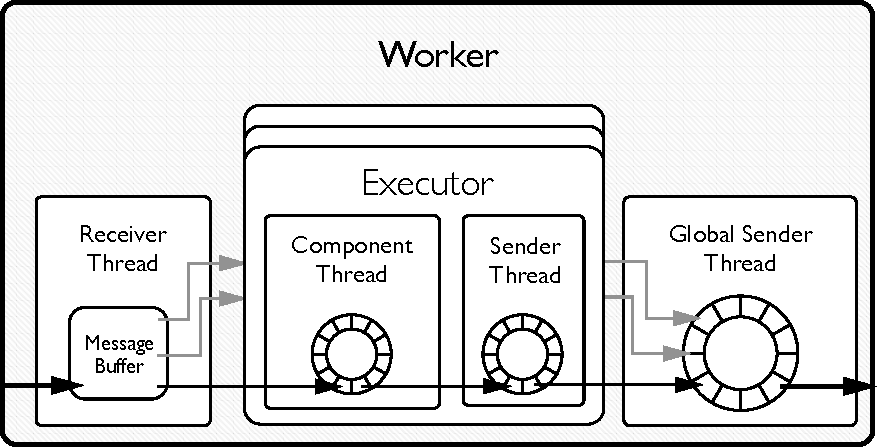
\includegraphics[scale=0.7]{pdf/worker_inside.pdf}
	\caption{Tuple processing in Apache Storm.}
	\label{fig:worker_inside}
\end{figure}

Figure \ref{fig:worker_inside} shows how tuple processing is implemented inside a Storm worker process. The tuple is read from a message buffer by the receiver thread of the worker and put on a receive queue of the target executor. The tuple is then picked up by the component thread of the executor for task execution.

After the component thread has executed the task it puts the tuple on the executor send queue. There, it is picked up by the executor sender thread which puts the tuple on the global send queue of the worker. Finally, the global sender thread of the worker serialises the tuple and sends it downstream.

Alternatively, if the tuple is forwarded to an executor in the same worker process it is put on the receive queue of the corresponding executor directly after task execution.

The queues used in Storm are implemented as ring buffers using the LMAX Disruptor library \citep{LMAXDisruptor}. Detailed background on how Disruptor works and its performance benchmarks can be found in \citep{Thompson_Farley_Barker_Gee_Stewart_2011}.

There is significant overhead required to simulate sending tuples to executors in other worker nodes. For one, there is the overhead from the tuple passing through the three queues of a worker. The authors of LMAX Disruptor showed that a three step pipeline has half the throughput of a single consumer-producer pipeline \citep{DisruptorWiki}.

Furthermore, to emulate over-the-network messages Storm uses a \texttt{Hashmap} of \texttt{LinkedBlockingQueue}s which according to \cite{Thompson_Farley_Barker_Gee_Stewart_2011} has several orders of magnitude lower performance than the Disruptor. Due to less write contention, lower concurrency overhead, and being more cache-friendly the Disruptor pattern can offer latency of inter-thread messages lower than 50 nanoseconds and a throughput of over 25 million messages per second \cite{Thompson_Farley_Barker_Gee_Stewart_2011}.

\subsection{Thread Overhead}

\begin{description}
	\item[Acker Bolt] \hfill \\
	The Acker bolt ensures that tuples propagate through a topology. In Storm it is included in every topology. It can be disabled via the configuration file in which case it is mostly idle since it does not receive any tuples. However, it can still use up resources especially if it waits fort tuples using a busy waiting strategy.
	\item[Heartbeats \& Timers] \hfill \\
	Every worker has a heartbeat thread that simulates sending heartbeat messages to the Nimbus node. It does this by writing to a local cache which is persisted to a file by a write on every heartbeat. Since the write is implemented using the \texttt{java.io} package the write is blocking - the thread cannot continue until the write is completed. While heartbeats are essential in cluster mode to signal the node being alive, there is no need for them in local mode.
	\item[Zookeeper Emulation] \hfill \\
	More overhead is produced by a local Zookeper server which emulates the Zookeeper nodes of a cluster. Running the Zookeeper server is a massive addition to the list of overheads as shown in the following paragraphs. The purpose of Zookeeper is to maintain states of running topologies and nodes of the cluster. As we will show in the following sections maintaining this state on multi-core is not necessary.
\end{description}

During profiling we found that a topology with one worker and three executors was being executed with 55 threads (not including system JVM threads and threads created by the profiler). Table \ref{table:breakdown} shows a breakdown of what the individual threads were used for.

\begin{table}[htb!]
\centering
\small
\begin{tabular}{@{}lc@{}}
    \textbf{Spout Parallelism} & \textbf{\# of Threads} \\ \toprule
    Main Thread & 1  \\
	Worker Sender \& Receiver Threads & 2  \\
    Acker \& System Component Threads & 2  \\
    Executor Component Threads & 3  \\
    Executor Sender Threads & 5  \\
    Various Timers \& Event Loops & 14  \\
    Zookeper Server & 28  \\
\end{tabular}
\caption[Storm thread usage]{Storm thread usage: topology with three executors.}
\label{table:breakdown}
\end{table}

To find out what state the threads were actually in at any given time the topology was executed for three minutes and a JVM thread dump was recorded every second. The average results of this experiment can be observed in table \ref{table:dump} and the state distribution over time can be seen in Figure \ref{fig:dump-plot}.

\begin{table}[htb!]
\centering
\small
\begin{tabular}{@{}lc@{}}
    \textbf{Spout Parallelism} & \textbf{\# of Threads} \\ \toprule
    RUNNABLE & 8  \\
	TIMED WAITING & 22  \\
    WAITING & 25  \\
\end{tabular}
\caption[Storm thread states]{Storm thread states: topology with three executors}
\label{table:dump}
\end{table}

<<dump-plot, echo=FALSE, cache=TRUE, fig.cap="Thread state distribution over time.", fig.pos="!htb", fig.height=3>>=
@

Even though three minutes may seem to be a short amount of time the fact that there is almost no variation shows that it is sufficient. As can be seen from the table, most of the threads were either in state \texttt{WAITING} or \texttt{TIMED WAITING}. According to the Java documentation on thread states \citep{JavaThreads} these two states are used for threads that are waiting for an action from a different thread and cannot be scheduled by the scheduler until that action is executed.

On average there were eight threads in state \texttt{RUNNABLE} which JVM uses to mark threads which are executing on the JVM and are possibly waiting for resources from the operating system (OS) such as processor \citep{JavaThreads}. Hence, these are threads directly competing to be scheduled by the OS. This means that for three components running in parallel there are five threads doing potentially unnecessary work.

In the subsequent sections we will show that these threads were in fact unnecessary and we will discuss how the number of threads was reduced. In fact, to execute the same topology on Storm-MC requires only 5 threads.

\section{Storm-MC Design}
\label{sec:storm_mc_arch}

The design we adopted for porting worker nodes is to only have one worker executing all the executors of a topology. This design simplified the communication model and allowed removal of unnecessary abstractions.

Additionally, the source code for the Nimbus service was merged with the worker source code. This was done because there is no need to run Nimbus and worker specific code in parallel. Once the Nimbus source code sets up the topology, all the work is done by the worker source code. Hence they can be executed serially.

\subsection{Porting Nimbus}

The role of Nimbus in Storm-MC has effectively been reduced to validating the topology and its configuration and passing the topology along to the worker source code which handles topology execution.

\subsection{Porting Worker Nodes}

In Apache Storm, a worker node runs a supervisor daemon, which in turns launches worker processes which run executors which execute tasks. There are thus three ways to control the parallelism of a component in Apache Storm: setting the number of workers, setting the number of executors per component, and setting the number of tasks per executor.

In Storm-MC, however, there is only one worker wrapper which runs all executors and their tasks - only one task executes within an executor. Hence, the parallelism of a component is controlled by only one variable: number of executors per component. This represents the number of threads that will function as the component within a topology. This design has several benefits:

\begin{itemize}
	\item All the communication occurs within one worker process.
	\item The supervisor daemon can be removed as there is no need to synchronise or monitor workers.
	\item There is no need to simulate over-the-network message passing.
	\item Message passing between executor threads within a worker stays the same as in Apache Storm.
\end{itemize}

A comparison of an Apache Storm worker node and its Storm-MC equivalent is shown in Figure \ref{fig:comparison}.

\begin{figure}[!htb]
\centering
\begin{subfigure}{.5\textwidth}
  \centering
  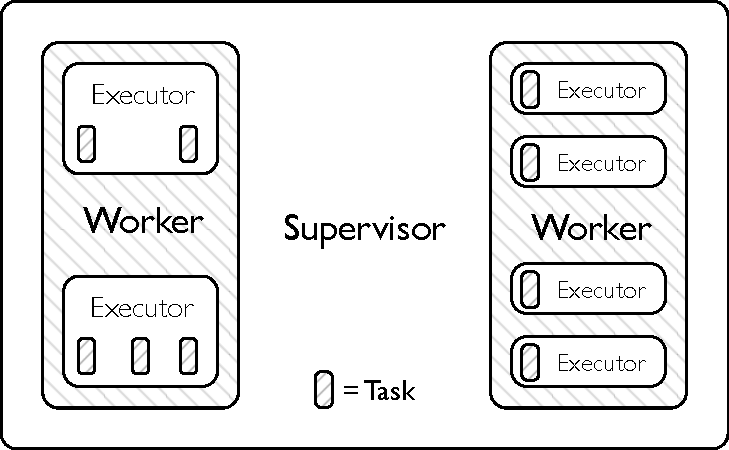
\includegraphics[width=0.95\linewidth]{pdf/distributed_worker.pdf}
  \caption{Worker node in Apache Storm.}
  \label{fig:comparison1}
\end{subfigure}%
\begin{subfigure}{.5\textwidth}
  \centering
  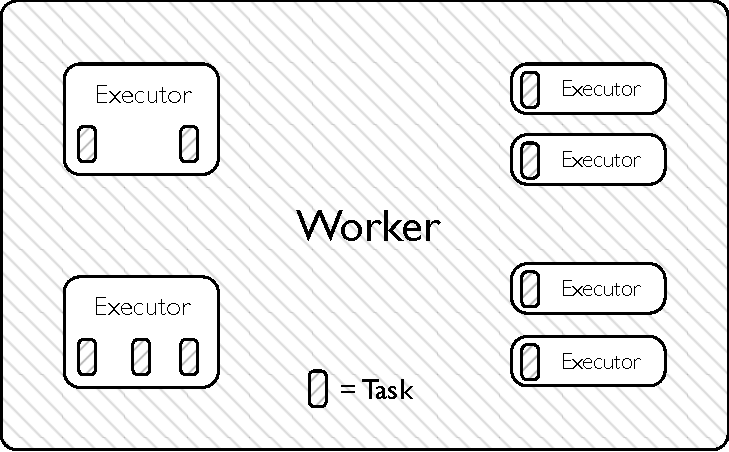
\includegraphics[width=0.95\linewidth]{pdf/local_worker.pdf}
  \caption{Worker node equivalent in Storm-MC.}
  \label{fig:comparison2}
\end{subfigure}
\caption{Comparison of a worker in Storm and Storm-MC}
\label{fig:comparison}
\end{figure}

The role of the worker wrapper is to launch executors and provide them with a shared context through which they can communicate. This is done with a map of Disruptor queues which the executors use as receive queues they pick tuples from.

Moreover, the worker wrapper contains a map of components and streams. This map specifies which bolts subscribe to a stream component produces. Executors use this map to figure out who they should send tuples to.

Additionally, the worker wrapper has a timer which components can use to get tick tuples at regular intervals. As mentioned before, bolts can use tick tuples to trigger events at regular intervals. For example, one might want to sort a window of tuples based on some criteria every five minutes.

Finally, a worker contains a configurable-size thread pool \texttt{ExecutorService}. Storm-MC executors can use this service via the topology context to launch background tasks on a shared thread pool.

\subsection{Removing State}

Storm-MC is completely stateless. The cluster state that was managed by Zookeeper in Apache Storm was completely stripped away. In Storm workers use the Zookeeper cluster state to communicate with Nimbus and vice versa. For example, when Nimbus creates topology assignments it informs workers via the cluster state. In Storm-MC, we adopted a more functional approach where worker is just a function invoked by the Nimbus part of the source code.

While this is not something that is visible to a user of Storm-MC, it required a great effort as all the code that used Zookeeper had to be refactored.

\subsection{Removing Serialisation}

Similarly to removing the Zookeeper state, great amount of work was put into removing the dependency of Storm-MC on Apache Thrift. This was mostly done to reduce code bloat and remove an unnecessary dependency since there is no serialisation required in a multi-core environment. Moreover, code generated by Thrift does not use standard Java camelCase naming conventions but instead uses underscore\_case. For example, Thrift generates method names such as \\ \texttt{get\_component\_common}.

This required refactoring all the data types generated automatically by Thrift. This not only reduced the size of the codebase significantly but also made the code more readable and self-documenting than the code generated by Thrift.

\section{Implementation Details}
\label{sec:implementation}

Most of the implementation was ported over from Storm-MC with adjustments where necessary. The problem with porting software is that there is a lot of functionality that needs to be changed but the changes required are usually not substantial. This section outlines details of Storm-MC implementation.

\subsection{Topology Submission}

Topologies are built using an instance of the \texttt{TopologyBuilder} class which uses the builder pattern - same as in Apache Storm. While the basis  of this class was reused from Storm, the internals had to be refactored so they work with data types used by Storm-MC. Once a topology is built it is submitted to an instance of \texttt{LocalCluster} class. This class is used in Storm for emulating the cluster on a local machine. Storm-MC adapted the class for backwards compatibility. This way, code created for Storm needs minimal adaptation to work on Storm-MC. A topology is submitted for execution via the \texttt{submitTopology} method which takes three arguments: the name of the topology, a Java Map with configuration, and a topology built by \texttt{TopologyBuilder}.

Users can submit a configuration file written in YAML. This is done by setting a JVM property called \texttt{storm.conf.file}. This file can for example define the capacity of the Disruptor queues, what waiting strategy should the components employ when there are no tuples to pick up, and what hooks they want executed every time a tuple is processed. Furthermore, users can define their own topology validator by implementing the \texttt{ITopologyValidator} interface.

\subsection{Tuple Processing}

\begin{figure}[!htb]
	\centering
	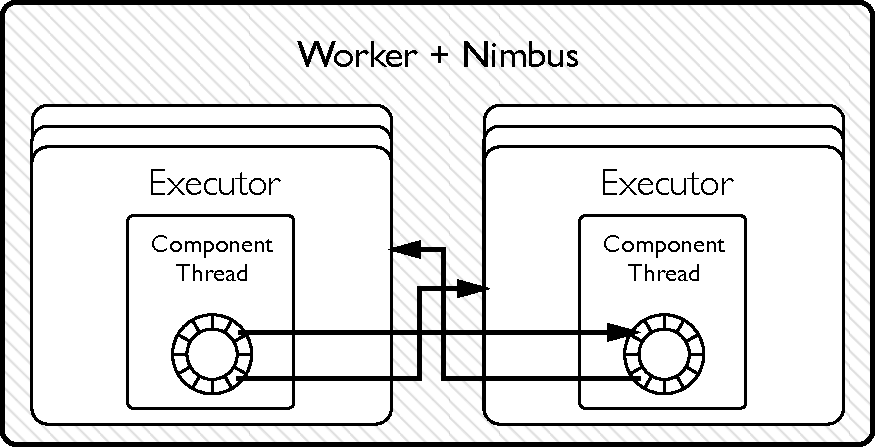
\includegraphics[scale=0.7]{pdf/worker_inside_mc.pdf}
	\caption{Tuple processing in Storm-MC.}
	\label{fig:worker_inside_mc}
\end{figure}

The implementation of tuple processing in Storm-MC is depicted in Figure \ref{fig:worker_inside_mc}. As can be seen from the figure, the queues used for remote message sending present in Storm were stripped away and there is only one Disruptor queue for every executor. Once an executor is done processing a tuple it puts it directly on the receive queue of its downstream bolts.

In Apache Storm, every executor runs two threads, one for tuple processing and one for tuple sending. In Storm-MC, however, there is only one thread per executor. Hence, the number of queues a tuple needs to pass through in a component is lowered as compared to Apache Storm.

Tuple processing in Storm-MC is a variant of multiple producer single consumer problem. In general, multiple producer single consumer problems are hard to optimise since there needs to be some form of synchronisation between multiple producers trying to produce an entry at the same time. In Disruptor queues this is implemented using the atomic Compare-and-Swap (CAS) operation. This operation ensures that even if multiple threads attempt to modify a variable only one of them succeeds and all threads involved are able to tell whether it was them that succeeded. Hence, one thread will succeed at claiming the next entry of a Disruptor queue and others will have to retry.

Alternatively, locks can be used used to synchronise access but lock-free queues using CAS are considered to be more efficient than locks because they do not require a kernel context switch \cite{Thompson_Farley_Barker_Gee_Stewart_2011}. However, even with CAS a processor must lock its instruction pipeline to ensure atomicity and employ a memory barrier to make the changes visible to other threads.

We investigated other data structures besides Disruptor queues that could be used for tuple exchange in Storm-MC but Disruptor queues are considered state of the art in low-latency parallel systems. This is one area that Apache Storm did really well and we were not able to further optimise.

Other options we considered were \texttt{ArrayBlockingQueue} and \texttt{LinkedBlockingQueue} both of which are in the Java standard library. However, the Disruptor shows superior throughput and latency compared to these options as shown in \citep{DisruptorWiki}.

\subsubsection{Waiting Strategies}

There are four different waiting strategies an executor can employ while waiting for a tuple to become available:

\begin{description}
	\item[BlockingWaitStrategy] \hfill \\
	This strategy uses a lock and a condition variable. The thread waits on the condition variable and is signalled once a new tuple becomes available. This strategy wastes the minimum number of CPU cycles when an executor is waiting.
	\item[SleepingWaitStrategy] \hfill \\
	This strategy initially spins for hundred iterations, then uses \texttt{Thread.yield()}, and finally uses \texttt{LockSupport.parkNanos(1L)} to sleep. Thus after quiet periods this strategy might introduce latency spikes.
	\item[YieldingWaitStrategy] \hfill \\
	This strategy initially spins for hundred iterations and then uses \texttt{Thread.yield()}. This strategy is a good compromise between CPU utilisation and great performance.
	\item[BusySpinWaitStrategy] \hfill \\
	In this strategy the thread is in a so-called tight loop, where it checks whether a new entry is available and only breaks out of the loop if there is a new entry. This strategy has the best performance but works well only if the number of CPU cores is higher than the number of active threads since it maximises CPU utilisation.
\end{description}

The default strategy used in Storm-MC is \texttt{BlockingWaitStrategy} but users can change the strategy in the configuration file.

\subsubsection{Tuple Pools}

Once a component wants to send a new tuple to its downstream components it needs to initialise a Java Tuple object. Here, we saw room for improvement since this might need to be done at very high rates, possibly million times per second.

Hence, a tuple pool was implemented where executors could place tuples after they were done with them so the tuples could be reused by other executors. However, access to this pool also had to be synchronised and hence accessing the pool introduced higher latency than simply initialising new tuples. Moreover, Java garbage collector actually does a good job of re-claiming unused memory and thus the idea of using a tuple pool was abandoned.

This problem could potentially be circumvented by using different constructs to achieve tuple passing but backwards compatibility with programs written for Apache Storm was deemed more important than the potential gain in performance.

\subsection{Executors}

The implementation of an executor processing a tuple is as follows:

\begin{enumerate}
	\item The executor repeatedly tries to pick a tuple from its Disruptor queue. If there are no tuples to be picked up it employs a waiting strategy between trials.
	\item Once it picks up a tuple, it processes it as per the component it represents.
	\item If it emits a new tuple it attempts to send it downstream by repeatedly trying to claim an entry of the downstream ring buffer.
	\item Once it successfully claims an entry it proceeds back to step 1.
\end{enumerate}

\section{Differences between Apache Storm and Storm-MC}
\label{sec:differences}

The codebase of Apache Storm is fairly large - 54,985 lines of code as reported by \texttt{cloc} \citep{Cloc}. Thus we had to prioritise features that were ported over to Storm-MC. Table \ref{table:features} presents a list of Storm features and shows which were ported over to Storm-MC and which were not.

\begin{table}[h!]
\centering
\small
\begin{tabular}{@{}lcc@{}}
    \textbf{Feature} & \textbf{Apache Storm} & \textbf{Storm-MC} \\ \toprule
    Multi-language Topologies & \cmark & \cmark \\
    Hooks & \cmark & \cmark \\
    Metrics & \cmark & \cmark \\
    Tick Tuples & \cmark & \cmark \\
    Multiple Topologies & \cmark & \xmark \\
    Topology Scheduling & \cmark & \xmark \\
	Trident API & \cmark & \xmark \\
    Built-in Metrics & \cmark & \xmark \\
    Nimbus as a Server & \cmark & \xmark \\
\end{tabular}
\caption{Feature comparison of Apache Storm and Storm-MC.}
\label{table:features}
\end{table}

A feature that we deemed very important is support for multi-language topologies. Thus, Storm-MC allows you to define components in other languages such as Python or Ruby and connect them into a Java topology. An example of a component defined in Python can be seen in Listing \ref{listing:wordcount_split_py}.

Storm-MC has support for task hooks just like Storm. Task hooks allow you to capture a number of events and execute custom code when the event occurs at a registered component. Hooks are created by subclassing \texttt{BaseTaskHook}. They can, for example, be used to update a web server with the latest performance metrics.

Additionally, Storm-MC has support for topology metrics. This way, components can record metrics such as number of tuples processed or a count of event occurrences. These metrics can then be automatically consumed by a bolt that subclasses the \texttt{MetricsConsumerBolt} class.

As mentioned before, Storm-MC supports tick tuples which can be used  to trigger component-local events at regular intervals.

Unlike Storm executing on a cluster, Storm-MC does not support running multiple topologies at the same time. However, to do that one only needs to run the topology in a separate process. This is because unlike when executing on the cluster different topologies do not need to share any state and it is more natural to execute them as separate processes. This design decision has the added benefit of each process having its own part of main memory thus reducing cache conflicts as shown in \citep{Chandra:2005:PIC:1042442.1043432} and providing higher security by not having different topologies share memory space.

Storm-MC does not support topology scheduling. Since within one process there is always only one topology running at a time and the hardware configuration of the machine does not change, the parallelism is clearly defined by the number of executors per component specified in the topology configuration.

One way to implement scheduling could be to pin threads to specific cores. Unfortunately, Java does not provide support for CPU affinity; the assignments are handled automatically by the JVM. Potentially, this could be achieved by using C or C++, both of which support CPU affinity, but this was not implemented in Storm-MC.

Apache Storm supports an alternative high-level API called Trident which then gets converted into spouts and bolts by the Storm library. Trident was omitted from Storm-MC but it would be possible to implement it on top of the current API.

Moreover, Apache Storm collects JVM metrics with a bolt called \texttt{SystemBolt}. This bolt is added automatically to all Storm topologies. This bolt is not included in Storm-MC topologies automatically but users can choose to add this bolt on their own.

Finally, Nimbus in Apache Storm performs as a server that clients can send topologies to for execution. In Storm-MC, we opted for a different design as outlined in previous sections. The interaction with the Nimbus service is usually through a shell script with a path to a JAR file of the topology and the main class to execute. This shell script was ported over to Storm-MC but instead of communicating with a service it spawns a new separate process that executes the topology.

